%!TEX root = ../main.tex

\chapter{Use Case}
\label{chp:usecase}

The proposed federated architecture in this thesis aims to run semantic queries over sparse and diverse data sources. In this chapter we will consider a practical use case of the architecture, showcasing both the flow of a query and its transformations among the diverse components of the architecture, as well as the inverse flow of the retrieved data, from the sources to the user interface.

\section{Experimental Setup}
The use case selected for this analysis involves a sophisticated \ac{SPARQL} query designed to interlink and analyze clinical and recording data from the \ac{BRAINTEASER} project dataset. This scenario is meticulously chosen to demonstrate the robust capability of the proposed architecture to manage and execute queries that necessitate access to multiple physical locations.
The experiment is structured to conduct a thorough examination of the various components comprising the architecture, beginning with an in-depth analysis of the query itself. This initial stage focuses on inspecting the query's structure, understanding how it interacts with the data sources, and predicting its flow through the underlying system components. The goal is to highlight the interaction between the query and the data layers, offering insights into the complexities involved in federated data management.
Following the structural analysis, the query's flow through the architecture will be meticulously presented and visualized. This involves analyzing each step of the query's execution, highlighting how it is rewritten, unfolded, and ultimately executed within the system. This phase aims to provide a clear and detailed schematic representation of the data flow, showcasing the dynamic interactions between the architectural components.
The final phase of the experimental setup involves the actual execution of the query. During this stage, we will closely monitor and document the transformations that the query undergoes at various stages of the architecture. From its initial transformation from \ac{SPARQL} into \ac{SQL} by the Ontop component, through its optimization and execution in the data virtualization layer powered by Dremio, each transformation will be presented.
The overarching objective of this experimental analysis is to validate the architecture's ability to efficiently manage and process complex queries across a federated data environment.

\section{SPARQL Query over ALSFRS Relations}
The selected \ac{SPARQL} query, presented in Code \ref{lst:sparql-alsfrs}, is specifically crafted to access and analyze the \ac{ALSFRS} data, which is crucial for assessing the progression of \ac{ALS} symptoms over time. This section discusses the structure of the query, its relevance to the dataset, and how it leverages the architecture's capabilities. The query employs the \ac{BRAINTEASER} ontology schema, indicated by the prefix bto, to query \ac{ALSFRS} data. It is designed to retrieve a comprehensive set of variables related to the \ac{ALSFRS} assessments, including total scores and sub scores for bulbar, motor, and respiratory functions, as well as individual question scores from the \ac{ALSFRS}-R (Revised \ac{ALS} Functional Rating Scale). 
This query not only fetches detailed patient assessment data but also organizes it chronologically for each patient, aiding in the longitudinal analysis of disease progression. The ordered structure facilitates efficient data retrieval and subsequent analysis in a clinical research context.
The chosen query is significant for several reasons: first and foremost, it accesses data unified from distinct sources, showcasing the architecture's capability to seamlessly integrate data across heterogeneous systems. Secondly, the query tests the system's capability to handle complex and extensive data structures, reflecting directly on the underlying data's relational union, which is a virtual view amalgamating identical table schemas from different databases. Finally, this same query will serve lately also as a benchmark to assess the correctness of the ontology mappings and the accuracy of data retrieval across the federated system. The ability to retrieve consistent and complete data sets across different platforms is crucial for validating the effectiveness of the federated architecture.
\begin{lstlisting}[language=SPARQL, caption={\ac{SPARQL} query on \ac{ALSFRS} visits performed by patients over the \ac{BRAINTEASER} ontology vocabulary}, label={lst:sparql-alsfrs}]
    PREFIX bto: <https://w3id.org/brainteaser/ontology/schema/>
    
    SELECT ?patient ?date ?tot ?bulbar ?motor ?respiratory ?q1 ?q2 ?q3 ?q4 ?q5 ?q6 ?q7 ?q8 ?q9 ?q10 ?q11 ?q12 WHERE { 
        ?p bto:undergo ?e.
        ?e bto:consists ?alsfrs.
        ?alsfrs a bto:ALSFRS;
               bto:procedureStart ?date;
               bto:revisedALSFRS ?tot;
               bto:bulbarSubscore ?bulbar;
               bto:motorSubscore ?motor;
               bto:respiratorySubscore ?respiratory;
               bto:alsfrs1 ?q1;
               bto:alsfrs2 ?q2;
               bto:alsfrs3 ?q3;
               bto:alsfrs4 ?q4;
               bto:alsfrs5 ?q5;
               bto:alsfrs6 ?q6;
               bto:alsfrs7 ?q7;
               bto:alsfrs8 ?q8;
               bto:alsfrs9 ?q9;
               bto:alsfrs10 ?q10;
               bto:alsfrs11 ?q11;
               bto:alsfrs12 ?q12.
        BIND(SUBSTR( (STR(?p)), 48) AS ?patient)
    } 
    ORDER BY ?patient ?date
\end{lstlisting}

\section{Query Flow}
The flow of the query from its original form to the actual data retrieval across physical data sources is a multi-step process involving several layers of translation and optimization. Each phase of this transformation leverages different components of the architecture to ensure accurate and efficient query execution. Figure \ref{fig:blockdiagram} represents in details this flow as the query is submitted to its final destinations (i.e. relational \ac{DBMS}s).
\subsection{Query Rewriting over Ontological Rules}
The first transformation step involves expanding the \ac{SPARQL} query according to the ontological rules defined in Ontop. Ontop uses these rules to interpret the query in the context of the ontology, enhancing the query by incorporating ontological knowledge. This includes inferring relationships, attributes, and classifications that are not explicitly stated in the query but are defined in the ontology. This expansion helps in making the query more comprehensive and aligned with the underlying data model, ensuring that the results are semantically consistent with the ontology's structure.
\subsection{Query Unfolding to SQL}
Once the query is expanded, Ontop performs the unfolding process. In this phase, the expanded \ac{SPARQL} query is translated into \ac{SQL} based on the mapping definitions that link the ontology to the virtual database schema. This step is crucial as it converts the high-level ontological query into a format that can be executed over a relational \ac{DBMS}. The unfolding process ensures that the query is syntactically correct and optimized for execution against the structured schema of the data sources. The syntactical correctness of the output \ac{SQL} query is strictly correlated with the correctness of the mappings.
\subsection{Execution of SQL on Virtual Views}
The final transformation occurs when the \ac{SQL} query is processed by Dremio, which acts on the virtual views defined over the physical data sources. Dremio takes the \ac{SQL} query and executes it against these virtual views, which represent a unified interface over the disparate databases. This phase is critical as Dremio optimizes the query's execution by deciding how best to access and retrieve the data from the underlying physical sources. This involves pushing down certain operations to the databases and merging results from the different sources.

\begin{figure}[ht]
    \centering
    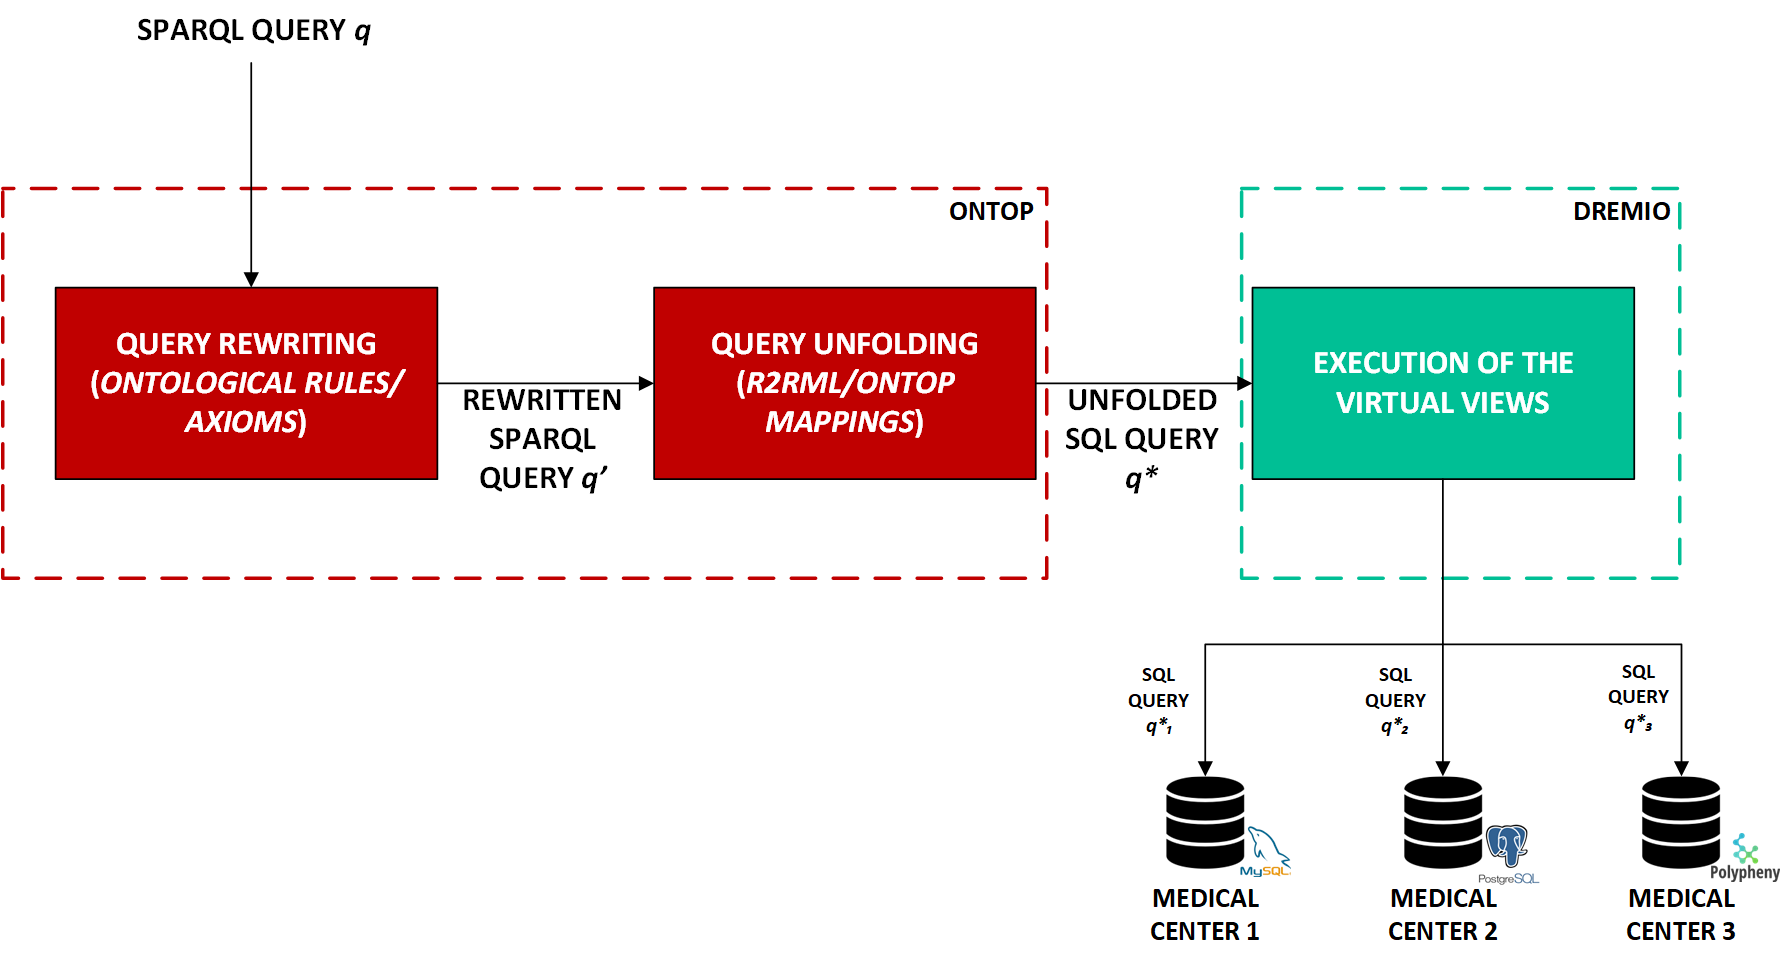
\includegraphics[width=15cm]{res/Drawing5.png}
    \caption{Data Flow Block Diagram of a Query Through the Federated Architecture}
    \label{fig:blockdiagram}
\end{figure}

\section{Exploration of Query Transformation in Ontop}
In this phase we are using the Ontop framework within the Protégé environment, specifically chosen for its debugging capabilities. This setup is ideal for detailed inspection and debugging of the query transformation process, from a \ac{SPARQL} query to an \ac{SQL} query executable on relational databases. This decision allows for a granular inspection of how queries are translated from \ac{SPARQL} to \ac{SQL}, focusing on the use of ontological rules and mappings. 
After setting up all the components, we ran the query and we waited for the retrieval process to be completed. Given the distribution and the heterogeneity of the sources, the process was time consuming with respect to high-performance, centralized \ac{DBMS}s. After assessing the result correctness by visual inspection, we analyzed the output query q* produced in output by the Ontop framework, that was submitted to Dremio.
The query resulted in having long recursive patterns, particularly due to special character parsing processes.
After manually inspecting and parsing these patterns in order to simplify and shorten the query repetitive body, we obtained the \ac{SQL} presented in \ref{lst:ontop-qstar}.
\begin{lstlisting}[language=SQL, caption={Parsed \ac{SQL} Translation of the Original \ac{SPARQL} Query}, label={lst:ontop-qstar}]
CONSTRUCT [patient, date, tot, bulbar, motor, respiratory, q1, q2, q3, q4, q5, q6, q7, q8, q9, q10, q11, q12]
   [date/RDF(CHARACTER VARYINGToVARCHAR(date2m51), xsd:datetime),
    q1/RDF(INTEGERToVARCHAR(q11m25), xsd:integer),
    motor/RDF(INTEGERToVARCHAR(motor1m55), xsd:integer),
    ...]
NATIVE
SELECT
    v23."bulbar1m17" AS "bulbar",
    v23."date2m51" AS "date",
    v23."motor1m55" AS "motor",
    v23."q101m44" AS "q10",
    v23."q111m42" AS "q11",
    v23."q11m25" AS "q1",
    v23."q121m41" AS "q12",
    v23."q21m24" AS "q2",
    v23."q31m23" AS "q3",

    --- ... more fields

    v23."patient26m9" AS "patient"
FROM (
    SELECT DISTINCT
        v7."bulbar" AS "bulbar1m17",
        v5."date2m51" AS "date2m51",
        v8."motor" AS "motor1m55",
        v1."patient" AS "patient26m9",
        v19."q10" AS "q101m44",
        v20."q11" AS "q111m42",
        v10."q1" AS "q11m25",

        --- ... more fields
        
        v6."tot" AS "tot1m45"
    FROM "clinical_data"."ALSFRS" v1
    
    --- ... recursive joins

    WHERE v1."patient" IS NOT NULL AND v1."date" IS NOT NULL
) v23

ORDER BY v23."date2m51" NULLS FIRST
\end{lstlisting}
The CONSTRUCT clause is crucial in shaping the structure of the resultant \ac{RDF} data, where each field is transformed to match a specific data type and linked to its \ac{RDF} representation. This transformation ensures that the output aligns with the expected semantic standards, facilitating subsequent data integration and analysis.
The NATIVE clause instead specifies the direct \ac{SQL} translation components, signifying how the translated query interfaces with the underlying \ac{SQL} database. It highlights the direct mapping of \ac{SPARQL} to \ac{SQL}, ensuring that the original semantic query's intent is preserved while being adapted for execution over relational data structures.
The SELECT clause in \ac{SQL} is constructed to directly map each variable specified in the \ac{SPARQL} SELECT query. Each variable such as ?patient, ?date, ?tot, etc., corresponds to specific fields in the underlying database tables. For example, bto:procedureStart translates to selecting the date column in \ac{SQL}. The \ac{SPARQL} BIND function used to extract the patient ID from a URL or string is represented in \ac{SQL} with a SUBSTRING function, allowing the extracted patient ID to be represented correctly in the result set.
The FROM clause in \ac{SQL} involves the specification of tables and joins that correspond to the triples patterns defined in the \ac{SPARQL} query. The \ac{SPARQL} predicate bto:undergo and bto:consists suggest relational joins between patient data and \ac{ALSFRS} assessment data. This relationship is mapped to \ac{SQL} joins or subqueries that fetch data from multiple related tables, capturing the relational nature of the data as specified by the ontology.
The WHERE clause in \ac{SQL} is essential for filtering data based on conditions expressed in \ac{SPARQL}. Conditions such as ensuring data completeness or filtering based on specific criteria (like date ranges or specific patient characteristics) are directly translated from \ac{SPARQL} conditions. The \ac{SQL} version ensures that only relevant, complete records are processed.
The ORDER BY clause in \ac{SQL} mirrors the \ac{SPARQL} order condition, ensuring that the results are returned in a specific order, which in this case is based on patient ID and date. This ordering is crucial for chronological analysis of patient data in medical research.
The detailed translation process showcases the precise alignment from \ac{SPARQL} to \ac{SQL}, ensuring that the data fetched and processed adheres strictly to the semantic structure defined by the ontology.

\section{Execution of q* on Dremio Virtual Views}
In our architecture, Dremio operates as a single-instance node rather than a distributed cluster, focusing on executing \ac{SQL} queries that have been transformed from \ac{SPARQL} to \ac{SQL}. This phase critically leverages Dremio's robust logging capabilities, which provide detailed insights into the query execution process. The Dremio query planner, which is central to its operation, allows for the export of query execution plans in \ac{JSON} format. By inspecting these logs, we can observe and analyze how the query is optimized and executed.
Dremio's execution engine processes the query against virtual datasets, which abstract the underlying physical data sources such as MySQL, PostgreSQL, and Polypheny. This virtualization allows for efficient data querying across heterogeneously structured data repositories without necessitating physical data aggregation or duplication. Such a setup is essential for maintaining high performance and flexibility in data handling.
The detailed query plan extracted from the \ac{JSON} log shows the optimizer's role in structuring the execution. It details the optimized execution paths designed to minimize the overhead associated with processing complex \ac{SQL} queries. These paths reflect the strategic planning of operations to enhance query performance by reducing unnecessary data shuffles and network traffic, which is crucial in a single-node setup where resource optimization is key.
The execution log provides insights into the handling of complex joins and the extensive use of URL encoding within \ac{SQL} queries. The presence of multiple nested SELECT statements and intricate joins illustrates Dremio's capability to reconstruct semantic relationships that were initially expressed in the \ac{SPARQL} format. This ensures that the semantic integrity and the meaning of the original queries are preserved and effectively adapted for execution over relational data structures.
Furthermore, the logs reveal Dremio's use of Apache Arrow for managing data formats, ensuring efficient data processing and exchange. This choice underscores the system's design towards maximizing processing speed and minimizing latency, which is particularly beneficial in a single-node environment where all processes converge on one machine.
Performance enhancement strategies such as sophisticated caching mechanisms are also evident from the logs. These mechanisms optimize the execution of repeated queries and manage frequently accessed data, thereby reducing execution times and improving the system's responsiveness.
Moreover, specific \ac{SQL} transformations highlighted in the log, including the decoding of URLs back to standard formats, underscore the meticulous attention to ensuring data compatibility and correctness. This aspect is critical for the subsequent stages of data analysis and integration.
By executing these virtual views, Dremio facilitates real-time data retrieval and analysis, crucial for dynamic decision-making processes in clinical research environments. The detailed inspection of Dremio's query execution logs not only demonstrates the practical application of semantic web technologies in modern data architectures but also ensures that the data retrieval process is both efficient and semantically consistent.

\section{Summary}
This chapter detailed a use case that applied our federated data analytics architecture to handle complex queries across diverse data sources. The architecture facilitated the integration and querying of heterogeneous data sets using \ac{SPARQL}-to-SQL translations within a federated system featuring Ontop and Dremio.
The experiment demonstrated the system's capability to efficiently manage and optimize complex queries, reducing execution times and maintaining data integrity. The analysis of Dremio's logs revealed effective query optimizations and the robust handling of federated queries, showcasing the potential of the architecture to support real-time, data-intensive operations in clinical genomics research.
Overall, the experiment confirmed the architecture's effectiveness in leveraging semantic web technologies and federated systems to enhance data processing and accessibility, setting a foundation for future research and applications in distributed data environments.